\documentclass[11pt,a4paper]{article}
\usepackage{graphicx}
\usepackage{geometry}
\geometry{margin=0.95in}
\usepackage{xcolor}
\usepackage{booktabs}
\usepackage{hyperref}
\hypersetup{colorlinks=true, urlcolor=cyan}
\pagestyle{empty}
\setlength{\parskip}{5pt}\setlength{\parindent}{0pt}

\begin{document}

{\LARGE \textbf{How the Language-Factor Share works}}\\[1.5mm]
{\small Waiz Khan (\texttt{wkhan12@jh.edu}). A plain-language guide to
the technical report. July 2026.}

\vspace{1mm}\hrule\vspace{3mm}

\textbf{The question it answers.} When a model reads the same sentence in
French and in Hindi, how much of its internal representation is about the
\emph{meaning}, and how much is about the \emph{language}? The
Language-Factor Share (LFS) is one number, between 0 and 1, that answers
this at every layer of a model. Near 0 means the model represents meaning
almost independently of language. Near 1 means representations cluster by
language, whatever the sentence says.

\textbf{Step 1: the data.} We use NTREX-128, a public benchmark in which
the same news sentences (about two thousand) were professionally
translated into 128 languages; we use 1{,}500 of them per language. Every sentence therefore exists in every language with the same
meaning. This gives us a grid: one axis is \emph{which sentence} (the
meaning), the other is \emph{which language}.

\textbf{Step 2: the representations.} Each sentence in each language is
passed through the model. At every layer, the model produces one vector per
token; we average these vectors over the sentence's tokens to obtain a
single sentence representation (the averaging is done in full numerical
precision; the two-event finding below was confirmed under a control that
matches the pooling across instruments, and a variant that corrects for
how finely each language's tokenizer splits words is queued as follow-up
work). The analysis is at the sentence level; word-level analysis through
alignment is planned follow-up work.

\textbf{Step 3: the decomposition.} With the grid of vectors in hand, we ask a bookkeeping question from analysis of variance: split the spread of the vectors into the parts each factor accounts for. Here the split is: how much of the spread between
representations is explained by \emph{which language} they came from, and
how much by \emph{which sentence} (which meaning)? LFS is the language
portion divided by the sum of both. Averaging vectors of the same sentence
across languages isolates meaning; averaging vectors of the same language
across sentences isolates language identity; comparing the spread of the
two gives the share.

\begin{center}
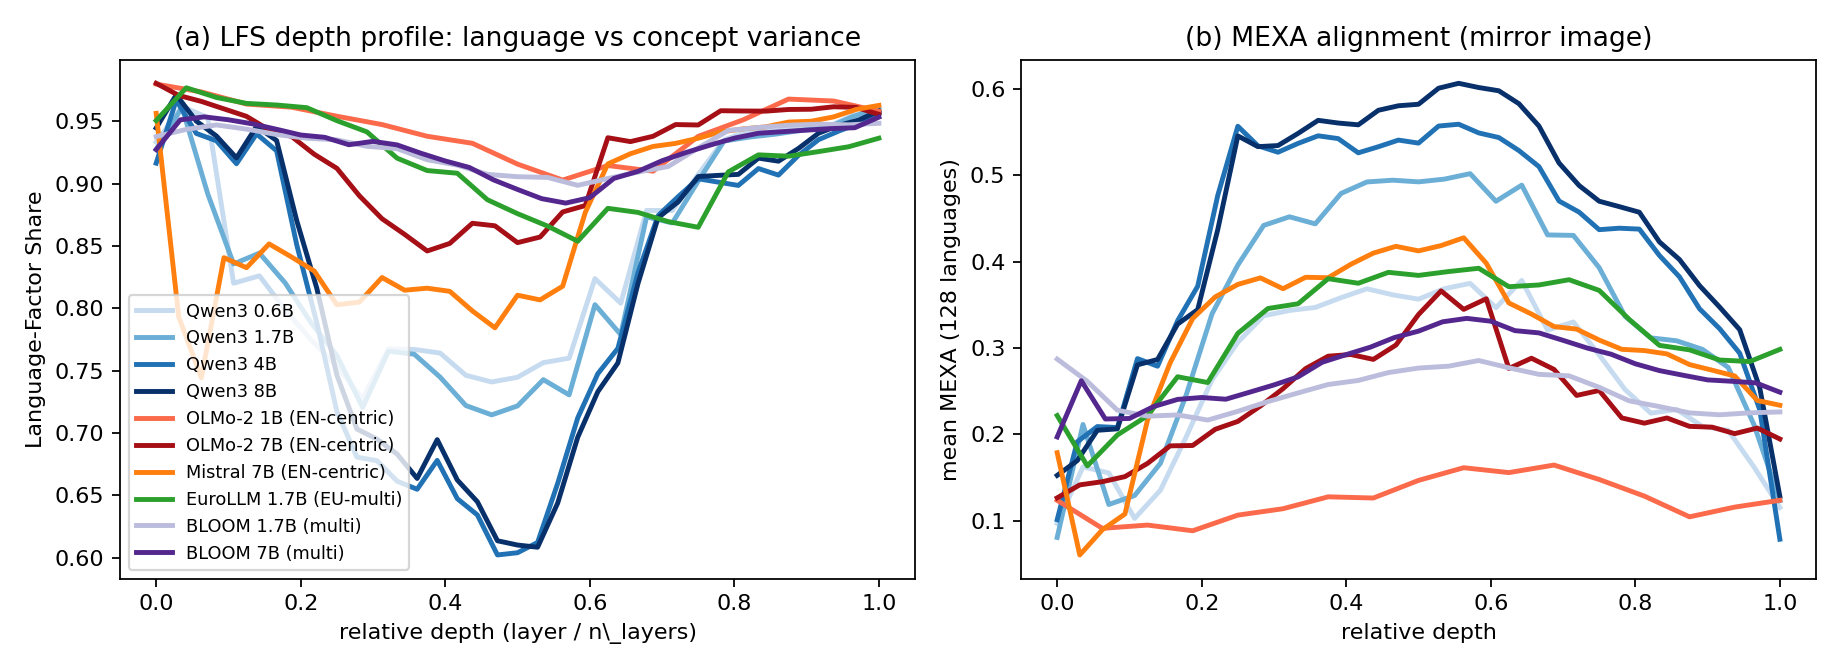
\includegraphics[width=0.9\textwidth]{figs/fig1_lfs_depth_profile.png}
\end{center}
{\small \textbf{What it looks like.} Every model shows the same shape:
representations start language-specific, become most shared in the middle
layers, and separate again toward the output. This shape is consistent
with the field's current understanding. What the measurement adds is that
the \emph{depth} of the shared region is a precise, comparable number: it
varies almost tenfold across seventeen open models (0.04 to 0.37), and it
turns out to depend more on how a model was trained than on how large it
is.}

\vspace{2mm}
\textbf{Why believe the number.} Three kinds of evidence, all collected
under predictions written down before the experiments ran. First, after
removing everything that data quantity, language family, writing system,
and tokenizer cost can explain, alignment measured at the LFS-selected
layer still relates to task performance, moderately (about 0.2 to 0.3 on the full grid after confound removal; an earlier benchmark-capable-subset figure of about 0.6 is withdrawn because it cannot be regenerated from a stored artifact); this is true of every intrinsic measure we computed, the published measure MEXA included.
Second, it predicts behavior: how much a model actually uses information
given to it in another language while generating text (0.67 after the same corrections on four models; 0.51 with a model-level interval of [0.19, 0.71] on a preregistered 19-model expansion across 13 families). Third, it generalizes: model families we had never touched
were classified correctly under a frozen protocol, blind.

\textbf{What it cannot do, measured rather than assumed.} We injected
known distortions into saved representations and checked what each
measure detects. The one structure LFS cannot attribute (rotation) turns
out to make up at most 0.7 percent of real cross-language differences. We
also found one way to fool every alignment measure we tested, including
the published measure MEXA: collapsing all representations toward a single
point. Only our accompanying check on concept spread detects it. That check
is now a required safeguard for any future training use.

\textbf{How it relates to published measures.} The closest existing measure (MEXA) asks whether
a sentence can find its translation among candidates; it is a useful
outside check and we report it throughout. LFS differs in three practical
ways: its value does not change with the size of the evaluation set, it
can be computed during training and differentiated, and it separates the
sources of cross-language difference rather than reporting a single
similarity. On predictive power after corrections the two are comparable;
the additional value of LFS is the decomposition and the safeguards
around it.

\vspace{1mm}\hrule\vspace{2mm}
{\small The accompanying technical report contains the methods,
statistics, comparisons, and error ledger behind each claim above.}

\end{document}
